\documentclass[12pt]{article}

\usepackage[utf8]{inputenc}
\usepackage[english]{babel}
\usepackage{natbib}
\usepackage[T1]{fontenc}
\usepackage{setspace}
\usepackage{graphicx}
\usepackage{hyperref}
\usepackage{float}
\usepackage[top=3.5cm,left=2.7cm,right=2.7cm,bottom=3.5cm]{geometry} % 'showframe' to see borders
\usepackage{booktabs}
\usepackage{subcaption}


\graphicspath{ {diagrams/} }

\title{\vspace{2cm}6G6Z1705\\\textbf{Artificial Intelligence}\\\vspace{2cm}Scenario 1\\\vspace{2cm}}
\author{14032908\\Joshua Michael Ephraim Bridge\\joshua.m.bridge@stu.mmu.ac.uk\\\vspace{1cm}}

\begin{document}

\maketitle

\newpage

\onehalfspacing

\section{Introduction}
In this report a process will be laid out which removes redundant parameters from images containing numeric digits using MATLAB \citep{matlab}. This includes reducing noise in the images and supplying information about the shapes. The data will then be input into WEKA \citep{hall2009weka} to distinguish between the different digits.

\section{Image Processing Methods}
  Noise within images distracts from classification, therefore it is vital to remove as much of it as possible. Below are some methods which will be used to remove noise / stabilise the images as a pre-step for other image encoding methods (section \ref{encoding}).

  \subsection{Scaling}
    The first chosen method for improving image data is through scaling of the image. While this method does not remove noise from the image, it allows other image processing / encoding methods to have more data points - such as creating a chain code (section \ref{chain-code}).

  \subsection{Gaussian Blurring} \label{sec:gauss-blur}
    A popular method for reducing noise is Gaussian smoothing. With this method a Gaussian kernel is applied as a convolution to pixel data which thereby produces a blurring effect on the image. This reduces grain noise but can also reduce detail within the image therefore a small standard deviation is key to not removing too much detail. Figure \ref{fig:gauss-filter} shows a Gaussian convolution applied to an image from the dataset with the Gaussian standard deviation set to 1.

    \begin{figure}[H]
      \begin{subfigure}{.5\textwidth}
        \centering
        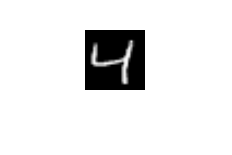
\includegraphics[width=0.5\textwidth]{scaled}
        \caption{Plain image}
        \label{fig:scaled}
      \end{subfigure}
      \begin{subfigure}{.5\textwidth}
        \centering
        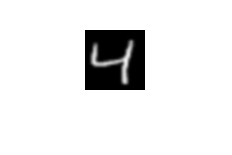
\includegraphics[width=0.5\textwidth]{blurred}
        \caption{Blurred image}
        \label{fig:blurred}
      \end{subfigure}
      \caption{Gaussian smoothing}
      \label{fig:gauss-filter}
    \end{figure}

  \subsection{Otsu thresholding} \label{otsu-thres}
    Creating a binary version of an image is a very useful tool for reducing noise. \cite{otsu1979threshold} presents a method which works by finding the threshold pixel value that minimises intra-class variance between black and white colours. Due to the removal of high variancy in pixel data it leaves a distinct binary shape which is much easier to extract shape information from, so long as there is not much noise in the image beforehand. An example of Otsu's method being applied to a Gaussian blurred image can be seen in figure \ref{fig:otsu-threshold}. Applying the thresholding method on top of Gaussian blurring ensures the resulting shape is smoother and has less noise around the shape edges.

    \begin{figure}[H]
      \begin{subfigure}{.5\textwidth}
        \centering
        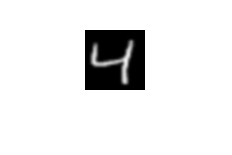
\includegraphics[width=0.5\textwidth]{blurred}
        \caption{Blurred image}
        \label{fig:blurred-2}
      \end{subfigure}
      \begin{subfigure}{.5\textwidth}
        \centering
        
\includegraphics[width=0.5\textwidth]{ohtsu}
        \caption{Thresholded image}
        \label{fig:ohtsu}
      \end{subfigure}
      \caption{Otsu thresholding}
      \label{fig:otsu-threshold}
    \end{figure}

  \subsection{Image eroding (edge finding)} \label{eroded}
    Finding the edges of shapes is a useful tool when creating a chain code (section \ref{chain-code}). \cite{haralick1987image} show that a good way to manipulate shape data is via morphological processing. In this case it will be used to erode the shape's size using a little cross as a kernel, then subtracting the eroded shape from the original will leave a border around the shape's edges (illustrated in figure \ref{fig:eroded}). Note that this requires the image to be in binary form which will be done via Otsu thresholding (section \ref{otsu-thres}).

    \begin{figure}[H]
      \centering
      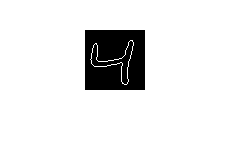
\includegraphics[width=0.25\linewidth]{edge}
      \caption{Shape edge after image erosion}
      \label{fig:eroded}
    \end{figure}

\section{Image Encoding methods} \label{encoding}
  Once as much noise / redundant information has been removed from the images as possible, it is then necessary to extract useful shape \& texture information which will aide the classifier in distinguishing between handwritten digits.

  \subsection{Chain Code} \label{chain-code}
   A chain code \citep{freeman1961encoding} is a very useful method for gathering shape information, especially for easily defined shapes such as handwritten digits which can be supplied in edge form. It works by taking in an image which has first been converted to an edge (section \ref{eroded}) and then describing the line information by splitting it into a series of connecting links with a direction value to the next link in the chain. Using the shape information provided by the chain code, other values about the shape can be calculated such as area, perimeter length and the shape compactness.

  \subsection{CCA (Connected Components Analysis)}
    CCA can be used to define the number and locations of multiple disconnected objects / shapes within an image (as shown by \cite{rosenfeld1966sequential}). It works by rastering the image multiple times and labelling different regions within the image, and determining connectedness by analysing neighbouring pixels. The CCA process should produce one feature vector per connected object provided that the image in question is made up of only binary objects \citep{cca}. This is useful in handwritten shape analysis as any identified disconnected shapes which are not useful can be discarded from analysis.

  \subsection{Co-occurrence matrices}
    In addition to shape information, textural information is also very useful to classification. Grey Level Co-occurrence Matrices is a form of textural co-occurrence analysis proposed by \cite{haralick1973textural}. It provides a textural mapping of pixel intensities throughout a gray image by comparing values at a given offset, up to a given pixel depth. In this report a horizontally neighbouring offset will be used with a pixel-depth value of 8.

  \subsection{Principal component analysis} \label{pca}
    Finally, principal component analysis \citep{pearson1901liii} will be used to reduce as much dimensionality in the output as possible. This will reduce the number of parameters by creating a statistical model of all training images \& creating a mean image for which every test image will be transformed into its variance from this mean model using only its principal distinguishing components. In comparison to direct pixel data this method will shrink the number of parameters immensely.

\section{Data classifiers} \label{classifiers}
  In the experimental stages of this report, three different classifiers will be tested for their suitability in classifying handwritten digits. The classifiers to be used will be the NaiveBayes, J48 and MultilayerPerceptron which are all implemented in WEKA \citep{hall2009weka}. An initial test will be done with all three, then one will be chosen on the basis of which gave the highest classification accuracy. Finally, the parameters for the chosen classifier will be optimised via a series of experiments to ensure the highest classification accuracy.

\section{Experimental Results}
  \subsection{Plan}
    Firstly, once every image processing \& encoding step has been completed an initial experiment will be run using the three different classifiers stated in section \ref{classifiers}. Further to this, some experimentation will be done with those processing steps to find the optimal configuration. Finally, once the optimal configuration is found, the best classifier will then be optimised with the output of the image processing in MATLAB in order to achieve the highest accuracy possible with the least redundant parameters.

  \subsection{Execution}
    Initially the output from MATLAB will comprise of (in this order):
    \begin{enumerate}
      \item Chain code descriptors (shape area, perimeter length, shape compactness)
      \item Co-occurrence matrices
      \item 10x10 scale version of image previously up-scaled to 60x60 pixels, Gaussian blurred with kernel size 1, then Otsu thresholded.
    \end{enumerate}
    The results from the classification of the output from this process are shown in table \ref{tab:blur1}, with each classifier using their default settings. Every following experiment will be a result of a small change from the settings just described (and used in table \ref{tab:blur1}), so as to use those results as a baseline.

    \newpage
    The first strategy is to alter the amount of blur placed on the images after up-scaling \& before thresholding. Table \ref{tab:blur} shows the differing accuracy scores when changing the Gaussian kernel sizes from 1 - 3. It is clear that a kernel size of 2 shown in table \ref{tab:blur3} gives the highest results on a MultilayerPerceptron, with a classification accuracy of 96.82\%.

    \begin{table}[H]
      \begin{subtable}{.329\linewidth}
        \centering
        \caption{Kernel size of 1}
        \begin{tabular}{c|c}
          \toprule
          \multicolumn{1}{c|}{Classifier} & \multicolumn{1}{c}{Accuracy (\%)} \\
          \midrule
          NaiveBayes & 75.31 \\
          J48   & 89.36 \\
          MLP   & \textbf{96.57} \\
          \bottomrule
        \end{tabular}%
        \label{tab:blur1}%
      \end{subtable}
      \begin{subtable}{.329\linewidth}
        \centering
        \caption{Kernel size of 2}
        \begin{tabular}{c|c}
          \toprule
          Classifier & Accuracy (\%) \\
          \midrule
          NaiveBayes & 76.45 \\
          J48   & 91.14 \\
          MLP   & \textbf{96.82} \\
          \bottomrule
        \end{tabular}%
        \label{tab:blur2}%
      \end{subtable}
      \begin{subtable}{.329\linewidth}
        \centering
        \caption{Kernel size of 3}
        \begin{tabular}{c|c}
          \toprule
          Classifier & Accuracy (\%) \\
          \midrule
          NaiveBayes & 85.94 \\
          J48   & 92.01 \\
          MLP   & \textbf{95.90} \\
          \bottomrule
        \end{tabular}%
        \label{tab:blur3}%
      \end{subtable}
      \caption{Changing Gaussian blur sizes (Default classifier parameters)}
      \label{tab:blur}
    \end{table}
    The next strategy is to alter the amount of up-scaling on the image before blurring \& thresholding, using a Gaussian kernel size of 1. Image sizes of 100x100, 60x60, 40x40 and  were tried, with results in tables \ref{tab:upscale-100}, \ref{tab:blur1}, and \ref{tab:upscale-40} respectively. The results show that an upscale to 60x60 pixels was the most effective with a MultilayerPerceptron classifier, which gave a score of 96.57\%.

    \begin{table}[H]
      \begin{subtable}{.5\linewidth}
        \centering
        \caption{Upscale image to 100x100}
        \begin{tabular}{c|c}
          \toprule
          \multicolumn{1}{c|}{Classifier} & \multicolumn{1}{c}{Accuracy (\%)} \\
          \midrule
          NaiveBayes & 74.17 \\
          J48   & 89.82 \\
          MLP   & \textbf{95.89} \\
          \bottomrule
        \end{tabular}%
        \label{tab:upscale-100}%
      \end{subtable}
      \begin{subtable}{.5\linewidth}
        \centering
        \caption{Upscale image to 40x40}
        \begin{tabular}{c|c}
        \toprule
        Classifier & Accuracy (\%) \\
        \midrule
        NaiveBayes & 86.53 \\
        J48   & 91.76 \\
        MLP   & \textbf{96.15} \\
        \bottomrule
        \end{tabular}%
        \label{tab:upscale-40}%
      \end{subtable}
      \caption{Changing up-scaling sizes (Default classifier parameters)}
      \label{tab:upscale}
    \end{table}
    The next strategy is to try outputting the shapes as their edges (section \ref{eroded}). The results in table \ref{tab:edges-only} show a clear degradation in classification accuracy from all classifiers when this action is performed, therefore this is not something which will selected for use in the final configuration.

    \begin{table}[H]
      \centering
      \begin{tabular}{c|c}
        \toprule
        Classifier & Accuracy (\%) \\
        \midrule
        NaiveBayes & 69.38 \\
        J48   & 70.11 \\
        MLP   & \textbf{76.30} \\
        \bottomrule
      \end{tabular}%
      \caption{Image as edges only (Default classifier parameters)}
      \label{tab:edges-only}%
    \end{table}%
    The next strategy is to try removing the shape \& textural encoding information to test if they are actually improving classification accuracy. Table \ref{tab:no-encoding} shows the results from removing both co-occurrence matrices and chain-code descriptors. The highest classifications from these scores do not exceed the baseline shown in table \ref{tab:blur1} therefore it can be inferred that the image encoding methods used do in fact increase discriminative power between digits.

    \begin{table}[H]
      \begin{subtable}{.5\linewidth}
        \centering
        \caption{Without co-occurrence matrices}
        \begin{tabular}{c|c}
          \toprule
          \multicolumn{1}{c|}{Classifier} & \multicolumn{1}{c}{Accuracy (\%)} \\
          \midrule
          NaiveBayes & 77.85 \\
          J48   & 88.51 \\
          MLP   & \textbf{96.10} \\
          \bottomrule
        \end{tabular}%
        \label{tab:no-co-occur}%
      \end{subtable}
      \begin{subtable}{.5\linewidth}
        \centering
        \caption{Without chain-code descriptors}
        \begin{tabular}{c|c}
        \toprule
        Classifier & Accuracy (\%) \\
        \midrule
        NaiveBayes & 87.31 \\
        J48   & 91.72 \\
        MLP   & \textbf{96.20} \\
        \bottomrule
        \end{tabular}%
        \label{tab:no-chain-code}%
      \end{subtable}
      \caption{Removing encoding data (Default classifier parameters)}
      \label{tab:no-encoding}
    \end{table}
    As a result of the previous experiments, an optimised classifier will now be produced which builds upon the highest classifying accuracy test completed in table \ref{tab:blur2} which shows a Gaussian kernel size of 2 has the best classification accuracy. As MultilayerPerceptron was the best performing classifier, the parameters of learning-rate, momentum and training time will be experimented with in order to produce a fully optimised classifier.\\

    Table \ref{tab:mlp-lr} shows the comparison of 5 different learning rate values, over a set of different training time values from 100 - 1000 epochs. Using the optimal training time of 200 from these results, a finer optimisation is carried out around the optimal learning rate parameter to ensure the accuracy given is the highest possible. This can be seen in table \ref{tab:mlp-lr-f} which shows that 0.5 is the most optimal value for learning rate.

    \begin{table}[H]
      \centering
      \begin{tabular}{c|ccccc}
        \toprule
              & \multicolumn{5}{c}{Learning Rate} \\
        \midrule
              & \multicolumn{1}{c|}{0.1} & \multicolumn{1}{c|}{0.3} & \multicolumn{1}{c|}{0.5} & \multicolumn{1}{c|}{0.7} & \multicolumn{1}{c}{0.9} \\
        \midrule
        \multicolumn{1}{l|}{Epochs} & \multicolumn{5}{c}{Accuracy (\%)} \\
        \midrule
        100   & 96.55 & 96.56 & 97.00 & \textbf{97.06} & 96.92 \\
        200   & 96.80 & 96.75 & \textbf{97.44} & 97.06 & 96.85 \\
        300   & 96.82 & 96.84 & \textbf{97.25} & 96.74 & 96.78 \\
        400   & 96.84 & 96.76 & \textbf{97.08} & 96.76 & 96.82 \\
        500   & 96.84 & 96.82 & \textbf{97.06} & 96.84 & 96.79 \\
        600   & 96.70 & 96.61 & \textbf{96.98} & 96.77 & 96.79 \\
        700   & 96.72 & 96.65 & \textbf{96.87} & 96.56 & 96.81 \\
        800   & 96.64 & 96.68 & \textbf{96.68} & 96.55 & 96.79 \\
        900   & 96.64 & 96.64 & \textbf{96.69} & 96.45 & 96.56 \\
        1000  & 96.56 & 96.62 & \textbf{96.69} & 96.57 & 96.60 \\
        \bottomrule
      \end{tabular}%
      \caption{Optimising MLP learning rate}
      \label{tab:mlp-lr}%
    \end{table}%

    \begin{table}[H]
      \centering
      \begin{tabular}{c|c}
        \toprule
        Learning Rate & Accuracy \\
        \midrule
        0.4   & 96.76 \\
        0.5   & \textbf{97.44} \\
        0.6   & 96.81 \\
        \bottomrule
      \end{tabular}%
      \caption{Finely optimising MLP learning rate (at 200 epochs)}      \label{tab:mlp-lr-f}%
    \end{table}%

    Next is to optimise the momentum parameter by performing a similar test to the one done in table \ref{tab:mlp-lr}, with a range of training times from 100 - 1000 epochs and 5 different values for momentum. Table \ref{tab:mlp-m} shows the results from these experiments. While the optimal value seems to vary over each different training time, it seems that a lower training time gives a higher accuracy therefore some more finely tuned experiments may identify the optimal values.

    \begin{table}[H]
      \centering
      \begin{tabular}{c|ccccc}
        \toprule
              & \multicolumn{5}{c}{Momentum} \\
        \midrule
              & \multicolumn{1}{c|}{0.1} & \multicolumn{1}{c|}{0.3} & \multicolumn{1}{c|}{0.5} & \multicolumn{1}{c|}{0.7} & 0.9 \\
        \midrule
        Epochs & \multicolumn{5}{c}{Accuracy (\%)} \\
        \midrule
        100   & 96.53 & 97.21 & \textbf{97.29} & 96.95 & 96.37 \\
        200   & 96.50 & 96.92 & 96.93 & 96.96 & \textbf{97.05} \\
        300   & 96.70 & 96.77 & 96.95 & 96.85 & \textbf{96.96} \\
        400   & 96.67 & 96.73 & \textbf{96.95} & 96.89 & 96.84 \\
        500   & \textbf{97.00} & 96.96 & 96.91 & 96.92 & \textbf{97.00} \\
        600   & \textbf{97.09} & 96.92 & 96.88 & 96.83 & 96.75 \\
        700   & 96.07 & \textbf{97.03} & 96.67 & 96.84 & 96.72 \\
        800   & \textbf{97.04} & 96.95 & 96.65 & 96.92 & 96.57 \\
        900   & \textbf{96.94} & 96.88 & 96.66 & 96.85 & 96.57 \\
        1000  & \textbf{96.89} & 96.86 & 96.66 & 96.62 & 96.64 \\
        \bottomrule
      \end{tabular}%
      \caption{Optimising MLP momentum}
      \label{tab:mlp-m}%
    \end{table}%

    Table \ref{tab:mlp-m-2} shows some fine tuning of momentum values at 100 \& 200 epochs and highlights a value of 0.2 at 200 epochs as the optimal value, with an accuracy of 97.44\%. Further to this, a more optimal training time can be found therefore a set of final experiments should be completed to find the most optimal possible classifier.

    \begin{table}[H]
      \centering
      \begin{tabular}{c|cccccccccc}
        \toprule
              & \multicolumn{10}{c}{Momentum} \\
        \midrule
              & \multicolumn{1}{c|}{0.1} & \multicolumn{1}{c|}{0.2} & \multicolumn{1}{c|}{0.3} & \multicolumn{1}{c|}{0.4} & \multicolumn{1}{c|}{0.5} & \multicolumn{1}{c|}{0.6} & \multicolumn{1}{c|}{0.7} & \multicolumn{1}{c|}{0.8} & \multicolumn{1}{c|}{0.9} & 1.0 \\
        \midrule
        Epochs & \multicolumn{10}{c}{Accuracy (\%)} \\
        \midrule
        100   & 96.53 & 97.00 & 97.21 & 96.98 & 97.29 & 96.98 & 96.95 & \textbf{97.25} & 96.37 & 9.82 \\
        200   & 96.50 & \textbf{97.44} & 96.92 & 96.86 & 96.93 & 96.82 & 96.96 & 96.90 & 97.05 & 9.82 \\
        \bottomrule
      \end{tabular}%
      \caption{Finely optimising MLP momentum}
      \label{tab:mlp-m-2}%
    \end{table}%

    Table \ref{tab:mlp-tt} shows the optimisation of the MLP training time with intervals of 10 epochs between tests, though no higher accuracy was found than at the already tested value of 200.

    \begin{table}[H]
      \begin{subtable}{.5\linewidth}
        \centering
        \caption{100 - 200 epochs}
        \begin{tabular}{c|c}
          \toprule
          Epochs & Accuracy (\%) \\
          \midrule
          100   & 97.00 \\
          110   & 97.03 \\
          120   & 97.24 \\
          130   & 97.24 \\
          140   & 97.28 \\
          150   & 97.28 \\
          160   & 97.30 \\
          170   & 97.33 \\
          180   & 97.23 \\
          190   & 97.36 \\
          200   & \textbf{97.44} \\
          \bottomrule
        \end{tabular}%
        \label{tab:mlp-tt-1}%
      \end{subtable}
      \begin{subtable}{.5\linewidth}
        \centering
        \caption{200 - 300 epochs}
        \begin{tabular}{c|c}
          \toprule
          Epochs & Accuracy (\%) \\
          \midrule
          200   & \textbf{97.44} \\
          210   & \textbf{97.44} \\
          220   & \textbf{97.44} \\
          230   & 97.37 \\
          240   & 97.30 \\
          250   & 97.27 \\
          260   & 97.30 \\
          270   & 97.33 \\
          280   & 97.30 \\
          290   & 97.26 \\
          300   & 97.25 \\
          \bottomrule
        \end{tabular}%
        \label{tab:mlp-tt-2}%
      \end{subtable}
      \caption{Optimising training time}
      \label{tab:mlp-tt}
    \end{table}%

\section{Conclusions}
  In conclusion, the best method defined in this report for classifying handwritten ‘4’ digits involves multiple image processing and encoding methods, and a classifier which is best suited for lots of parameters with highly varying values. Below the best methods discovered in this report will be laid out.

  \subsection{Image processing methods} \label{improc}
    The best image processing method found seems to be a combination of three different processes. The first is increasing resolution of the image to 60x60 pixels (just over 4 times the number of pixels from 28x28). The next step seems to be smoothing this scaled image using a Gaussian kernel size of 2 (see table \ref{tab:blur2}). Finally, thresholding the image to produce a binary version of the shape seems to be much better than when just a shape as edges is used (see table \ref{tab:edges-only}).

  \subsection{Image encoding methods} \label{imenc}
    The best image encoding methods described in this report are the chain code and co-occurrence matrices. Both of these perform well in increasing discriminative power between the digits, as seen in table \ref{tab:no-encoding}. Furthermore using PCA \ref{pca} reduces the output size of the processing steps greatly and decreases the time taken for classification.

  \subsection{Classification methods} \label{imcls}
    By far the best classifier in this task is the MultilayerPerceptron. Due to its capability of having a large structure which deals well with many parameters with abstract connections between the parameters. In this case the hidden layer structure was left at default settings which is the number of parameters $+$ the number of classes in a single hidden layer.

  \subsection{Discussion}
    The results found in this paper explore a few different ways of reducing dimensionality \& improving discriminative power between digits. What this report does not achieve is a comprehensive comparison of a wide range of many image processing \& encoding methods and their various combinations. This would be beyond the scope of this report however many other techniques exist which could be beneficial in the task of recognising digits. Some examples of other methods include wavelet representation \citep{mallat1989theory}, ‘moments’ which describe the shape's layout \citep{hu1962visual}, or many others described by \cite{zhang2004review}.\\
    The recommendation by this report is the combination of image processing, encoding and classification techniques described in sections \ref{improc}, \ref{imenc} \& \ref{imcls} respectively for use in reducing dimensionality and increasing discriminative power when classifying between handwritten ‘4’ digits and all others.

\newpage

\bibliographystyle{agsm}
\bibliography{report-nick}

\end{document}
